%\documentclass[conference,spanish,a4paper,10pt,oneside,final]{IEEEtran}
\nonstopmode
\documentclass[conference,spanish,a4paper,10pt,oneside,final]{tfmpd}


% esto me setea la variable pdf dependiendo del valor de \pdfoutput, que es >0
% sólo cuando estoy usando pdflatex para compilar el documento
\newif\ifpdf
\ifnum\pdfoutput<0
\pdffalse\fi
\ifnum\pdfoutput=0
\pdffalse\fi
\ifnum\pdfoutput>0
\pdftrue\fi

%\makeatletter
%\def\markboth#1#2{\def\leftmark{\@IEEEcompsoconly{\sffamily}\MakeUppercase{\protect#1}}%
%\def\rightmark{\@IEEEcompsoconly{\sffamily}\MakeUppercase{\protect#2}}}
%\makeatother


%
% ===
% === I18n / L10n
% ===
%
% babel me da separación de sílabas para palabras en el idioma que le paso como
%       argumento opcional. <-- Éste hay que pasarlo en \documentclass
%\usepackage{babel}
%
% inputenc define la codificación de caracteres del código fuente, acá utf8.
\usepackage[utf8]{inputenc}
%
% ===
% === Gráficos
% ===
% 
% pst-pdf me permite usar PSTricks con pdflatex. Necesito cargarlo sólo si está
%         definida la variable pdf, por eso está entre \ifpdf ... \fi
\ifpdf\usepackage{pst-pdf}\fi
%
% color me permite usar colores en el documento.
\usepackage{color}
%
% graphicx me da el comando \includegraphics para insertar imágenes (?)
\usepackage{graphicx}
%
% pstricks es un conjunto de macros basadas en PostScript para TeX, en
%          castellano, me da un entorno pstricks y comandos que uso dentro de
%          éste, que me sirven para dibujar figuras/diagramas/etc de manera
%          relativamente simple.
%\usepackage{pstricks}
%
% pst-circ me da macros para pstricks que me dibujan elementos de circuitos
%\usepackage{pst-circ}
%
% 
%\usepackage{pst-plot}		%Para dibujar una curva a partir de un archivo
%\usepackage{pst-2dplot}		%Para plotear. entorno pstaxes
%
% ===
% === Verbatims
% ===
%
% verbatim es una reimplementación de los entornos verbatim[*]
%          provee el comando \verbatiminput{archivo} y el entorno comment, que
%          hace que LaTeX ignore directamente todo lo que está adentro
%\usepackage{verbatim}
%
% moreverb implementa el entorno verbatimtab indentando los tabs que encuentre,
%          y también el entorno listing, que pone números de línea al verbatim.
%          Para cambiar el ancho de la tabulacion, uso
%          \renewcommand\verbatimtabsize{<ancho del tab>\relax}
%          También define el entorno boxedverbatim.
%\usepackage{moreverb}
%
% listings me da el entorno lstlisting con resaltado de sintaxis.
%          Para setear el lenguaje del código, hago \lstset{language=<lang>}
%\usepackage{listings}
%
% url es un verbatim para escribir URL's que permite linebreaks dentro de ésta.
%     para usarlo, \url{<URL>}
\usepackage{url}
%
%
%
%
%
%\usepackage{mdwlist}		%Para listas mas compactas
%\usepackage{textcomp}		%Para algunos símbolos
%\usepackage{colortbl}		%Para celdas de colores en tablas
%\usepackage{fancyhdr}		%Para encabezados/pie
%\usepackage{bbold}		%Fuente bb para modo math: \mathbb{R} = reales
%\usepackage{dsfont}		%Fuente ds para modo math: \mathds{R} = reales
\usepackage{multirow}		%Para "combinar" celdas en tablas
%\usepackage{float}		%Para cuadros, figuras, etc copadas
%\usepackage{fancybox}		%Para recuardos de texto con bordes "fancy"
%\usepackage{dingbat}		%Para dingbats
%%\usepackage{marginal}		%Para notas al margen que no puedo hacer andar
\usepackage{amsmath}		%Para enornos matemáticos mas flexibles
%\usepackage{varwidth}		%varwidth es un minipage que se ajusta al ancho mínimo
\usepackage{pslatex}            % setea fuentes Times, Helvetica y Courier ``angosta''

\usepackage[normalem]{ulem}     %para under/overlining. normalem hace que \emph se comporte como siempre

%
% Propiedades del documento: título, autor, etc
%
%% \newcommand{\titulo}{{\large FICH --- UNL}\\Procesamiento Digital de Imágenes
%% 2010\\Trabajo Final}
%% \newcommand{\autor}{Fornal, Esteban \and Pfarher, Christian \and Torrez, Mauro}
%% \newcommand{\fecha}{\today}
%% \newcommand{\tituloPDF}{Trabajo Final PDI 2010}
%% \newcommand{\autorPDF}{Fornal, Pfarher, Torrez}
%% \newcommand{\asuntoPDF}{}
%% \newcommand{\clavesPDF}{}
%

%Estilos de texto
\newcommand{\resalt}{\colorbox{green}}	%Resaltado - Fondo verde
\newcommand{\sfbf}{\bfseries\textsf}	%Slanted + Bold
\newcommand{\eng}{\textit}			%Palabra en inglés - Itálica
\newcommand{\mean}{\textsl}			%Significado de una sigla - Slanted
\newcommand{\defin}{\textbf}			%Definición - Negrita
\newcommand{\R}{\mathds}			%Para escribir R de Reales, N de Nat
\newcommand{\N}{\mathbf}			%Para escribir R de Reales, N de Nat
\newcommand{\lil}[1]{\footnotesize #1}
\newcommand{\mono}[1]{{\tt #1}}         % Monoespaciado


%Símbolos
\newcommand{\y}{\wedge}			%Y (Lógica)
\newcommand{\ve}{\vee}			%O (Lógica)
\newcommand{\ent}{\supset}		%Entonces (Lógica)
\newcommand{\dimp}{\leftrightarrow}	%Doble implicativo, equivalencia (Lógica)
\newcommand{\sii}{\leftrightarrow}	%Si y sólo si (Lógica)
\newcommand{\equi}{\equiv}		%Equivalencia (Lógica)
\newcommand{\portanto}{\vdash}	%Por lo tanto (Lógica)
\newcommand{\por}{\cdot}		%Producto punto

%Configuraciones del documento
%\selectlanguage{spanish}		%Elijo idioma español

%Tweaks
%\setlength{\parindent}{0mm}		%Sangría de 1a. línea
%\setlength{\hoffset}{-5.4mm}		%
%\setlength{\voffset}{-5.4mm}		%
%\setlength{\topmargin}{0mm}		%
%\setlength{\oddsidemargin}{5mm}	%
%\setlength{\evensidemargin}{5mm}	%
%\setlength{\marginparsep}{5mm}	%
%\setlength{\headheight}{12.5mm}	%
%\setlength{\headsep}{2.5mm}		%
%\setlength{\footskip}{10mm}		%
%\setlength{\textwidth}{15cm}		%
%\setlength{\textheight}{232mm}	%
%\setlength{\fboxrule}{.1pt}
%\setlength{\parskip}{.5\baselineskip}
%Colores
\definecolor{negro}	{cmyk}{0,0,0,1}
\definecolor{marron}	{cmyk}{0,.5,1,.41}
\definecolor{rojo}	{cmyk}{0,1,1,0}
\definecolor{naranja}	{cmyk}{0,.35,1,0}
\definecolor{amarillo}	{cmyk}{0,0,1,0}
\definecolor{verde}	{cmyk}{1,0,1,0}
\definecolor{azul}	{cmyk}{1,1,0,0}
\definecolor{violeta}	{cmyk}{.45,1,0,0}
\definecolor{gris}	{cmyk}{0,0,0,.5}
\definecolor{blanco}	{cmyk}{0,0,0,0}
\definecolor{dorado}	{cmyk}{0,.16,1,0}
\definecolor{plateado}	{cmyk}{0,0,0,.25}

%Comandos personalizados
\newcommand{\T}{\textrm}%Para escribir texto común cuando en modo math

% Remarca un ``texto insertado'' en rojo. Necesita el backage color.
\newenvironment{ins}{\color{red}$>$}{$<$}
\newcommand{\iins}[1]{{\color{red}$>$#1$<$}}

% Tacha un texto. Depende del package ulem.
\newcommand{\tachar}{\sout}

% Tacha doble
\newcommand{\Tachar}[1]{\xout{\xout{#1}}}

%\newcommand{\}

%\begin{pspicture}
%\def\tierra(#1){%Para dibujar el símbolo de tierra en el entorno PSTricks
%	\rput(#1){
%		\psdot(0,0)
%		\psline(0,0)(0,-0.45)
%		\psline(-0.5,-0.45)(0.5,-0.45)
%		\psline(-0.35,-0.6)(0.35,-0.6)
%		\psline(-0.2,-0.75)(0.2,-0.75)
%	}%
%}
%\end{pspicture}

%\newcommand{\codigo}[2]{%Para generar un recuadro con código
%	%\setlength{\hrulewidth}{0.1pt}
%	\begin{flushleft}
%	\underline{#1}
%	\begin{tabular}{@{\quad}|l}
%		\begin{minipage}{.85\textwidth}\smallskip{#2}
%	\end{minipage}\end{tabular}\end{flushleft}%
%}

%\newcommand{\filecodigo}[1]{%Insertar código verbatim desde un archivo
%\codigo{#1}{\verbatiminput{#1}}}%Requiere el paquete verbatim
%\newcommand{\filecodigobis}[1]{{\verbatiminput{#1}}}%Requiere el paquete verbatim

%\newcommand{\grafico}[3][1]{%Para generar un plot de un archivo con coords.
%%\def\deequis=#1
%\begin{minipage}{0.5\textwidth}\begin{center}
%\begin{pspicture}(6,5)
%	\psgrid[subgriddiv=1,gridlabels=0pt,gridwidth=.1pt](1,3)(1,1)(6,5)
%	\psset{xunit=5cm,yunit=2cm}
%	\fileplot[linewidth=1pt,linecolor=blue,origin={0.2,1.5}]{#2}
%	\psset{xunit=1cm,yunit=1cm}
%	\psaxes[Dx=#1,dx=5,Oy=-1,Dy=1,dy=2]{-}(0.9,1)(6,5)
%	\rput(4,0.4){\textsl{#3}}
%\end{pspicture}\end{center}\end{minipage}}

%\newcommand{\aclaracion}[1]{%Dibuja un recuadrito aclaratorio
%\smallpencil\ \begin{minipage}{0.9\textwidth}
%\vspace*{6pt}{#1}\smallskip\end{minipage}}

%\newcommand{\consigna}[1]{%Consigna - Slanted
%\leftpointright\ \parbox[t]{0.9\textwidth}{\textsl{#1}\vspace{8pt}}}

%\newcommand{\pinterno}[2]{%Consigna - Slanted
%\left\langle #1 , #2 \right\rangle}

%\newcommand{\eqncode}[2]{%
%\begin{center}
%\begin{tabular}{l@{\hspace{0.5cm}}r}
%\begin{minipage}{.4\textwidth}
%\begin{equation*}
%#1
%\end{equation*}
%\end{minipage}
%&
%\fbox{\begin{minipage}{.4\textwidth}
%%\setlength{\parskip}{4mm}
%\filecodigobis{#2}
%\end{minipage}}
%\end{tabular}
%\end{center}
%}

%\newcommand{\eqncodeb}[2]{%
%\begin{center}\begin{tabular}{l@{\hspace{0.5cm}}r}
%\begin{minipage}{.4\textwidth}#1\end{minipage} &
%\fbox{\begin{minipage}{.4\textwidth}\filecodigobis{#2}\end{minipage}}
%\end{tabular}\end{center}}

%\newenvironment{matemcode}[1]{\newline
%\begin{tabular}{l@{\hspace{0.5cm}}r}
%\begin{minipage}{.4\textwidth}
%\parbox[t]{.4\textwidth}{\begin{equation*}#1\end{equation*}}\end{minipage}
%&\begin{Sbox}\begin{minipage}{.4\textwidth}}
%{\end{minipage}\end{Sbox}\fbox{\TheSbox}\end{tabular}\newline}

%\newenvironment{encuadrar}[1]{\begin{Sbox}\begin{varwidth}{#1\textwidth}}
%{\end{varwidth}\end{Sbox}\fbox{\TheSbox}}

%\newenvironment{enunciado}
%{\leftpointright\ \begin{varwidth}[t]{0.9\textwidth}\textsl}
%{\end{varwidth}\vspace{8pt}}

%\newenvironment{parboxenv}{\begin{Sbox}}
%{\end{Sbox}\parbox[t]{.9\textwidth}{\TheSbox}}

%\newenvironment{pvi}{\begin{equation*}\begin{cases}}
%{\end{cases}\end{equation*}}

% Escribe el texto que le paso como parámetro con letra de ancho fijo.
%\newcommand{\mono}[1]{{\tt #1}}

%\title{\titulo}
%\author{\autor}
%\date{\fecha}

%% si uso pdflatex, me setea las propiedades del pdf de salida
%\ifpdf\pdfinfo{/Title    (\tituloPDF)
%               /Author   (\autorPDF)
%               /Subject  (\asuntoPDF)
%               /Keywords (\clavesPDF)}\fi

%\include{conf/comandos}
%
\begin{document}
\title{Reconocimiento de edificios y monumentos}
\author{Fornal Esteban, Pfarher Christian, Torrez Mauro\\
\textit{Trabajo práctico final de ``Procesamiento Digital de
Imágenes'', II-FICH-UNL.}}
\markboth{Procesamiento Digital de Imágenes: TRABAJO FINAL}{}
\maketitle
%
%
% %%%%%%%%%%%%%%%%%%%%%%%%%%%%%%%%%%%%%%%%%%%%%%%%%%%%%%%%%%%%%%%%%%%%%%%%%%%%%%
%
%
\begin{abstract}
El objetivo de este trabajo consiste en la identificación de edificios y monumentos, a partir de imágenes obtenidas mediante un dispositivo móvil de características estándar en el mercado. Para dicho propósito se plantearán dos métodos diferentes, uno mediante extracción de características en el espacio de la Transformada de Hough y otro basado en medidas estadísticas, comparando a cada uno de ellos por separado y finalmente, evaluando el desempeño de la utilización de ambos conjuntamente.
\end{abstract}
%
%
% %%%%%%%%%%%%%%%%%%%%%%%%%%%%%%%%%%%%%%%%%%%%%%%%%%%%%%%%%%%%%%%%%%%%%%%%%%%%%%
%
%
\begin{keywords}
Identificación de edificios, detección de edificios, \eng{building recognition}, identificación de monumentos
\end{keywords}
%
%
% %%%%%%%%%%%%%%%%%%%%%%%%%%%%%%%%%%%%%%%%%%%%%%%%%%%%%%%%%%%%%%%%%%%%%%%%%%%%%%
%
%
\section{Introducción}
\PARstart{L}{a} presencia de gran cantidad de dispositivos tecnológicos de diferente índole ha abierto un sin número de nuevas aplicaciones para satisfacer las necesidades diarias de seres humanos. Los dispositivos móviles como celulares, PDAs, etc. han pasado a formar parte del común de nuestras vidas brindando nuevas posibilidades de interacción. Es aquí donde surge la idea de la realización de este trabajo. 
Día a día, las personas toman fotografías de diferentes objetos ya sean monumentos públicos, edificios históricos, etc. sin saber si quiera que se está fotografiando. Con este artículo se trata de hacer un aporte en vías hacia dicho problema, de manera que mediante el procesamiento de imágenes se tenga dicha información en el instante mismo de la adquisición de la foto.
En principio y ya que no es el objetivo de este trabajo hacer un análisis profundo, sino tan solo dar una aproximación inicial a la resolución del problema, se considerará la aplicación de los métodos en condiciones ideales o semi-ideales, \resalt {esto es en condiciones ambientales normales (sin ningún tipo de factores climáticos....}
%
%
% %%%%%%%%%%%%%%%%%%%%%%%%%%%%%%%%%%%%%%%%%%%%%%%%%%%%%%%%%%%%%%%%%%%%%%%%%%%%%%
%
%
\section{Método propuesto}
Se desarrollaron dos algoritmos diferentes para la resolución del problema.
%Una FAM es un sistema borroso que codifica \emph{mapeos} o transformaciones entre
%conjuntos borrosos. 
%
%El tipo de FAM más simple es aquella que mapea la regla $(A_i,B_i)$, la cual asocia
%el conjunto borroso $p-$dimensional $B_i$ con el conjunto $n-$dimensonal $A_i$.
%En general, un sistema FAM $F: I^n \rightarrow I^p$ codifica una serie de $m$ reglas
%$(A_1,B_1),\ldots,(A_m,B_m)$.
%
%Como cada conjunto representa una cantidad en lenguaje corriente, el conjunto de
%reglas en la FAM se define en torno a una asociación lngüística simple, por ejemplo,
%$($FRESCO$,$BAJO$)$ podría indicar una relación temperatura $\rightarrow$ nivel del
%calefactor.
%
%%\resalt{TODO: indicar cuál es la relación entre $A$ y los $A_i$.}
%
%Dada una entrada real $x$ al sistema, obtendremos una serie de valores de
%pertenencia $\mu_{A_{i}}(x), 0\leq\mu_{A_{i}}\leq1$, para cada conjunto de entrada $A_i$, que en la
%FAM activa cada regla en diferentes grados;
%al evaluar la regla $(A_i,B_i)$, se obtiene $B'_i$,
%una versión de $B_i$ parcialmente activado.
%Cuanto mayor sea el valor $\mu_{A_{i}}(x)$, más parecido será $B'_i$ a $B_i$.
%
%El conjunto $B$ de salida se obtiene mediante un promedio ponderado de los
%conjuntos parcialmente activados $B'_1,B'_2,\ldots,B'_m$:
%\begin{equation}
%B=w_1B'_1+\cdots+w_mB'_m
%\end{equation}
%donde $w_i$ es un grado certeza, o frecuencia, de la asociación $(A_i,B_i)$.
%En la práctica, se \emph{defuzzifica} comúnmente la salida $B$ a un único
%valor real $y$ mediante el método de los centroides, según
%\begin{equation}
%y=\frac{\sum_{i=1}^{m}{a_ic_i}}{\sum_{i=1}^{m}{a_i}}
%\end{equation}
%donde $a_i,c_i$ son el área y centroide, respectivamente, del conjunto $B'_i$ parcialmente
%activado.
%
%De esta forma podemos obtener para una entrada $x$ la salida $y$ del sistema [1].
\subsection*{Método mediante Transformada de Hough}
no se porque corno no anda lo de abajo.. ver...
%\begin{figure}
%\includegraphics[scale=0.1]{../diagramas/procesohough.ps} 
%\caption{"Proceso de la imagen mediante el método por T. de Hough}
%\end{figure}
%\subsection*{Método estadístico}
%
%
% %%%%%%%%%%%%%%%%%%%%%%%%%%%%%%%%%%%%%%%%%%%%%%%%%%%%%%%%%%%%%%%%%%%%%%%%%%%%%%
%
%
\section{Experimentos y resultados}
blablabla
%Partiendo de una implementación base de un juego de carrera de autos, 
%%que rebautizamos
%%como ``Fuzzy Driver'',
%la extendimos codificando una serie de \emph{sensores} montados en
%el auto, que devuelven un ``voltaje'' en un rango $\in [0,1]$, los cuales sensan
%la distancia a otros autos, en línea recta: emiten una señal de $1V$ cuando
%la distancia es máxima, y de $0V$ cuando es mínima (hay algo ``tocando'').
%Hemos elegido este rango de valores con el propósito de obtener generalidad.
%
%Los sensores frontales se ubican justo al lado de los faros del auto, de tal
%forma que están orientados hacia adelante, y se ubica además un sensor a la 
%derecha y otro a la izquierda, apuntando a los laterales.
%Los sensores laterales trabajan en un rango de distancias distinto al de los
%frontales, y suponemos que son capaces de detectar, además de autos, la
%banquina de la pista.
%
%El controlador consiste en dos módulos FAM, uno  comanda la dirección
%del volante, y el otro la aceleración y frenado, como se ve en la figura 1.
%%
%\begin{figure}[tbhp]
%%\centerline{\includegraphics[width=7cm]{img/diag-modulos}}
%\caption{Diagrama funcional del controlador.}
%\label{fig1}
%\end{figure}
%%
\subsection{Descripción de la Base de datos de imágenes}
Las imágenes sobre las cuál se aplicarán los algoritmos, fueron tomadas en la ciudad de Santa Fe, mediante un Dispositivo Móvil con una resolución de 640x480 pixels. Se construyo una base de datos de imágenes sobre 6 edificios, tomando 13 realizaciones de cada uno de ellos (10 con el propósito de usarlas como prototipo y 3 para la prueba con los algoritmos).
%El módulo de dirección lee las entradas
%\mono{dis\-tan\-cia\_fron\-tal\_iz\-quier\-da}, \mono{dis\-tan\-cia\_fron\-tal\_de\-re\-cha},
%\mono{dis\-tan\-cia\_la\-te\-ral\_iz\-quier\-da}, y \mono{dis\-tan\-cia\_la\-te\-ral\_de\-re\-cha},
%de los respactivos sensores, las fuzzifica, aplica las reglas FAM y
%calcula el valor de salida \mono{di\-rec\-ción\_vo\-lan\-te}, que está en el rango
%$[-1,1]$. El actuador tornea el volante a la izquierda cuando el valor
%es negativo, a la derecha cuando es positivo, lo mantiene centrado cuando
%el voltaje de salida es 0.
%
%El módulo de aceleración y frenado tiene las entradas \mono{ve\-lo\-ci\-dad\_ac\-tual},
%\mono{dis\-tan\-cia\_fron\-tal\_máxi\-ma}, y \mono{dis\-tan\-cia\_fron\-tal\_mí\-ni\-ma}, donde
%estas dos últimas son la máxima y mínima medida en los sensores frontales. De
%esta manera se logra simetría en las decisiones en este módulo. Las salidas
%son dos, \mono{aceleración} y \mono{frenado}, ambas variando de 0 a 1, donde 0
%indica no pisar el pedal, y 1, pisarlo a fondo.
%
%Para obtener las salidas de ambas FAM se utiliza el método de defuzzificación
%por centroides, como se describió antes, y los conjuntos de salida son como
%se ve en la figura \ref{fig3}. Los conjuntos de fuzzificación para las 
%entradas se pueden ver en la figura \ref{fig2}. 
%%
%\begin{figure}[tbhp]
%%\centerline{\includegraphics[width=6cm]{img/conj-entradas}}
%\caption{Conjuntos borrosos para fuzzificación de las entradas.}
%\label{fig2}
%\end{figure}
%%
%\begin{figure}[tbhp]
%%\centerline{\includegraphics[width=6cm]{img/conj-salidas}}
%\caption{Conjuntos borrosos para defuzzificación de las salidas.}
%\label{fig3}
%\end{figure}
%%
\subsection{Descripción de pruebas}
blablabla
%Para obtener las reglas nos hemos basado en proposiciones en lenguaje natural,
%como puede ser ``si la distancia medida por los dos sensores frontales es máxima, y
%la velocidad actual es media, entonces pisar a fondo el acelerador''. 
%
%La codificación utilizada es la de correlación-mínimo, la regla $(A_1\y A_2\y A_3,B_2)$
%se activa una cantidad $a$ dada por
%\begin{equation}
%a=\T{mín}(a_1(x),a_2(x),a_3(x))
%\end{equation}
%donde $a_i$ indica el grado de activación del conjunto $A_i$. 
%
%
% %%%%%%%%%%%%%%%%%%%%%%%%%%%%%%%%%%%%%%%%%%%%%%%%%%%%%%%%%%%%%%%%%%%%%%%%%%%%%%
%
%
\subsection{Tablas}
\begin{tabular}{cc}
\hline columna1 & columna2 \\ 
\hline  &  \\ 
\hline 
\end{tabular} 

%
%
% %%%%%%%%%%%%%%%%%%%%%%%%%%%%%%%%%%%%%%%%%%%%%%%%%%%%%%%%%%%%%%%%%%%%%%%%%%%%%%
%
%
\subsection{Discusión}
blablabla
%
%
% %%%%%%%%%%%%%%%%%%%%%%%%%%%%%%%%%%%%%%%%%%%%%%%%%%%%%%%%%%%%%%%%%%%%%%%%%%%%%%
%
%
%La evaluación del controlador borroso se realizó utilizando dos conjuntos de reglas
%y comparando su performance con la de jugadores humanos.
%
%En el primer conjunto de reglas borrosas (CR1) utilizado se pretende describir un comportamiento similar al de
%de un jugador humano que intenta esquivar a los demás coches en la pista con la menor
%disminución posible en la velocidad. 
%
%Mediante modificaciones en dichas reglas se logró un segundo conjunto de
%reglas (CR2) que modela el comportamiento de un conductor conservador que intenta
%esquivar al resto de los coches evitando velocidades altas y movimientos pronunciados. 
%
%Los parámetros evaluados fueron: la cantidad de colisiones, la distancia total recorrida en píxeles 
%y el tiempo fuera de pista.
%Se realizaron simulaciones de 3 minutos cada una utilizando una combinación de 5 y 10 competidores
%simultáneos (máximo) manejados por un controlador difuso (CD) igual al del coche principal, y también otros con movimiento 
%vertical uniforme (MVU) a su velocidad máxima. En todos los casos la velocidad máxima
%de los competidores se eligió de forma aleatoria
%entre 300 y 700 píxeles por segundo, mientras que la del coche principal fue fija
%y de 500 píxeles por segundo.

%Para evaluar la distancia total recorrida se utilizo el producto de la velocidad instantánea por el diferencial de tiempo
%transcurrido en intervalos pequeños.

%original  Se consideró al coche principal como fuera de la pista cuando un porcentaje del mismo mayor al 30\%
% se encontraba fuera de la misma.
%maurete modif
%Se consideró al coche principal como fuera de la pista cuando más del 30\% de éste se encontraba fuera de la misma.
%%
%Para cada una de las pruebas de los controladores se realizaron 3 simulaciones y se promediaron sus resultados.
%Para obtener medidas de la performance de jugadores humanos (JH) se promediaron los tiempos
%de dos jugadores.
%
%\begin{figure}[tbhp]
%%\centerline{\includegraphics[width=5cm]{img/evaluacion}}
%\caption{Resultados de la evaluacion del controlador borroso para (a) cantidad de colisiones,
% (b) distancia recorrida,  (c) tiempo fuera de la pista.}
%\label{evaluacion}
%\end{figure}
%
%En la figura \ref{evaluacion}(a) pueden observarse los resultados obtenidos respecto a la cantidad de colisiones. 
%En todos los casos, éstas aumentaron con un mayor número de competidores. En general, se registraron menos colisiones con los
%competidores MVU. Con 10 competidores el CR1 mostró una cantidad de colisiones levemente menor que los JH.
%En todos los casos el CR2 logró en general una mejor performance.
%
%La distancia recorrida total (figura \ref{evaluacion} (b)) fue, en todos los casos, mayor con los JH.
%El CR2 registró las menores distancias, y en la totalidad de los casos se registraron mayores distancias con competidores
%MVU y con un menor número de competidores.
%
%Al medir el tiempo fuera de pista (figura \ref{evaluacion} (c)),
%con 10 competidores, CR2 y JH registraron tiempos similares. En todos los
%casos el CR1 registró los mayores tiempos fuera de pista. Con 5 competidores los tiempos registrados fueron
%menores que con 10 competidores, y las diferencias más marcados, siendo JH el que menor tiempo fuera de pista registró
%y el conjunto de reglas 2 con tiempos un poco mayores.
%
%La implementación rudimentaria de los sensores resulta el principal cuello de botella a la hora de obtener
%entradas de calidad para la FAM, y trunca las posibilidades a la hora de plantear las reglas del controlador borroso.
%El jugador humano es capaz de percibir dichas entradas y además utilizarla para realizar procesos
%de razonamiento muy complejos y difíciles de modelar, que le permiten obtener respuestas mucho mejor ajustadas
%al resultado que se espera lograr.
%
%Además, existen otros factores como el juicio de valor que puede hacerse
%respecto a una situación determinada. Por ejemplo si se trata de rebasar
%un auto pero el único lugar es saliendo de la pista, puede elegir
%rebasarlo por la banquina para no perder velocidad, o no esquivarlo y frenar para no chocarlo.
%A pesar de ello, la performance obtenida por el controlador es equiparable en varios aspectos a la de un jugador humano
%medianamente experimentado. 
%
%Finalmente, en la figura \ref{evaluacion}(a) se observa un bajo número de colisiones para el CR2,
%excepto en el caso de 5 competidores MVU donde dicho valor es drásticamente alto.
%Esto puede ser atribuido una situación puntual que representa una limitación inherente a la implementación de los sensores.
%Dicha situación ocurre cuando se intenta rebasar un auto cercano a la banquina por la misma dirección de esta última.
%Las reglas que dicen que el coche debe esquivar y que no debe salir de la pista se contradicen y éste nunca puede rebasar
%al competidor y continúa chocándolo repetidamente desde atrás en cada intento.
%
%
% %%%%%%%%%%%%%%%%%%%%%%%%%%%%%%%%%%%%%%%%%%%%%%%%%%%%%%%%%%%%%%%%%%%%%%%%%%%%%%
%
%
\section{Conclusiones}
blablabla
%Hemos presentado un... sistema de control borroso para un piloto automático en un videojuego
%de carrera de autos sencillo. El uso de FAMs permite la especificación de las reglas
%en forma directa mediante proposiciones lingüístcas. 
%El rendimiento del controlador fue bueno, considerando la sencillez de especificación
%de las reglas y la muy baja complejidad de los sensores, los resultados han sido comparables
%a los de un jugador humano.
%
%Este modelo de controlador puede ser fácilmente implementable para manejar los competidores
%en un juego de carreras más complejo, dotando a éste de mayor parecido con la realidad, ya
%que simula bastante bien conductores humanos. Se deberá considerar en este caso la implementación
%de, al menos, un sensor de velocidad lateral y mejorar la disposición y número de sensores frontales.
%
%Los sensores utilizados en la
%implementación no difieren en mucho de detectores reales disponibles en el mercado,
%sin embargo, se deberán agregar sensores más complejos, muy posiblemente algún clasificador
%mediante una red neuronal y elaborar reglas con criterios
%minuciosamente verificados antes de llevar un controlador de este tipo a una implementación
%en un automóvil real, ya que evitar colisiones o salirse de pista no es una opción en el
%mundo real.
%
%
% %%%%%%%%%%%%%%%%%%%%%%%%%%%%%%%%%%%%%%%%%%%%%%%%%%%%%%%%%%%%%%%%%%%%%%%%%%%%%%
%
%
\section{Trabajos futuros}
A partir del diseño aquí presentado, seguiremos investigando esta técnica con las siguientes
posibilidades:
\begin{itemize}
\item blablabla
\end{itemize}

\nocite{*}
\bibliographystyle{tfmpd}
\bibliography{tfmpd}
\end{document}

